\documentclass{bredelebeamer}


\begin{document}

\title[INFO-F-410 - Traffic Light Control]{\textbf{Traffic Light Control} \\INFO-F-410 -- Embedded Systems Design} % The short title appears at the bottom of every slide, the full title is only on the title page

\author[]{Jamal \textsc{Ben Azouze}, Marien \textsc{Bourguignon}, Nicolas \textsc{De Groote}, \\Simon \textsc{Picard}, Arnaud \textsc{Rosette}, Gabriel \textsc{Ekanga}}
\institute[ULB] % Your institution as it will appear on the bottom of every slide, may be shorthand to save space
{
Université Libre de Bruxelles \\ % Your institution for the title page
\medskip
\textit{Département d'Informatique} % Your email address
}
\date{4 Juin 2015} % Date, can be changed to a custom date

\begin{frame}
\titlepage % Print the title page as the first slide
\end{frame}

\begin{frame}{Sommaire}
\tableofcontents % Throughout your presentation, if you choose to use \section{} and \subsection{} commands, these will automatically be printed on this slide as an overview of your presentation
\end{frame}

\section{Introduction}
\begin{frame}{First idea}
\centering
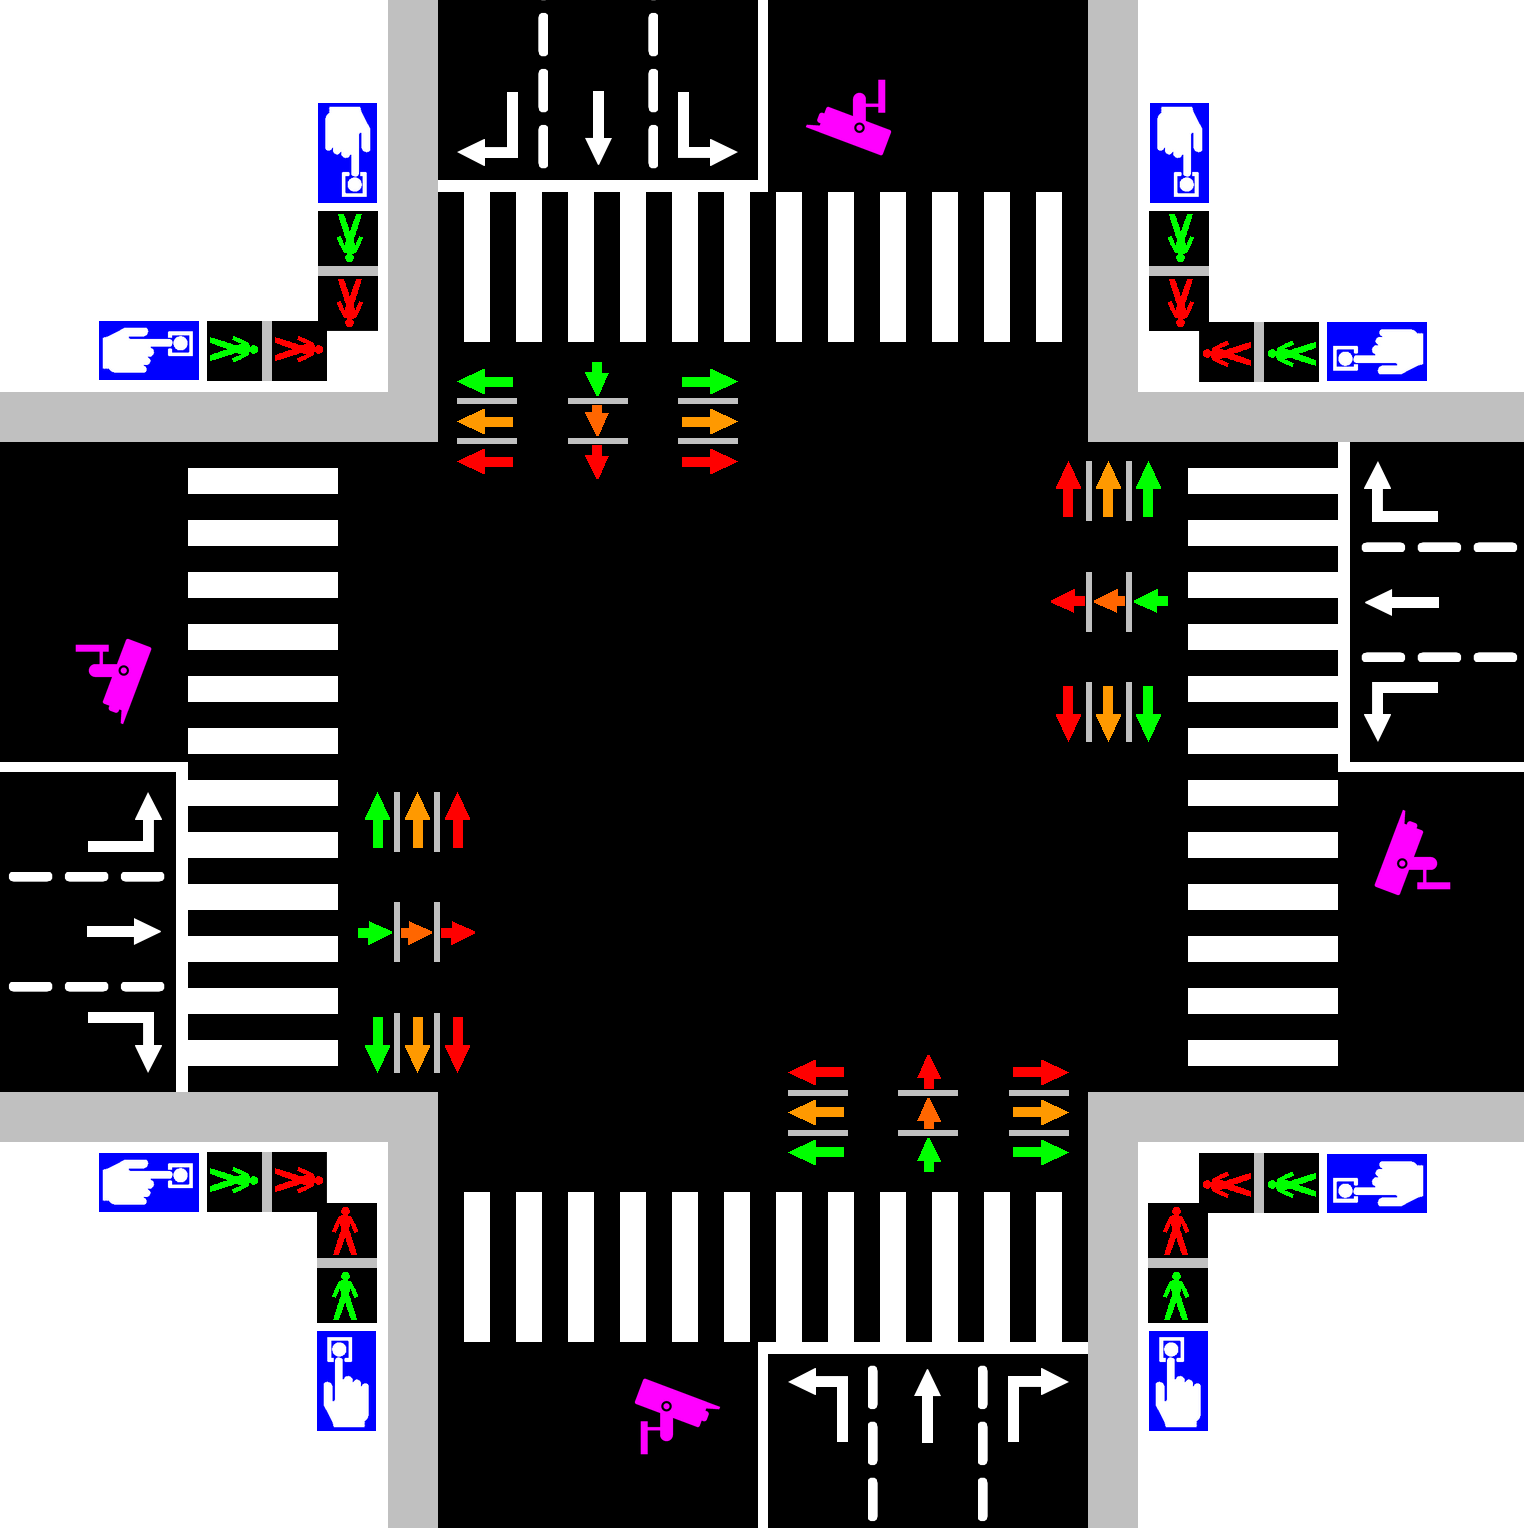
\includegraphics[scale=0.15]{images/idea_draft.png}
\end{frame}
\begin{frame}{Refined idea}
\centering
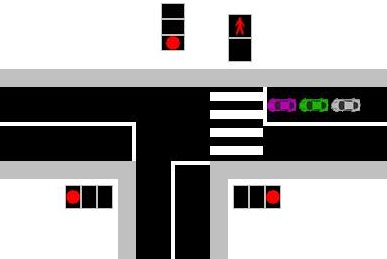
\includegraphics[scale=0.8]{images/final_idea.png}
\end{frame}

\begin{frame}{Assumptions}
\begin{itemize}
\item The traffic lights do not have orange lights -> cars stop instantaneously
\item Every entity respect the highway code 
\item At any time a car can arrive and join a queue of cars
\item At any time a pedestrian can push the button to cross the street
\item A pedestrian will always cross the street in less than a fixed time
\item A car will always cross the crossroads in less than a fixed time
\end{itemize}
\end{frame}

%Est-ce-qu'on fait une slide sur le lien avec embedded system?

%\begin{frame}{Joint project with Embedded System course}

%\end{frame}


\begin{frame}{Embedded System}
 \begin{itemize}
\item Lives are at stake -> Critical system
\item Impossible to test manually every combination -> Use of winning strategies
\end{itemize}
\centering
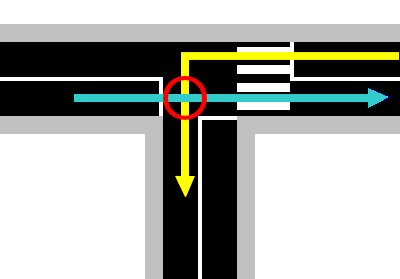
\includegraphics[scale=0.4]{images/exempleCollision.png}
\end{frame}

\section{Actors and automatons}
\begin{frame}{Actors}
\begin{enumerate}
\item <1-> Pedestrians
\item <2-> Cars
\item <3-> Traffic lights
\end{enumerate}
\end{frame}

\begin{frame}{Pedestrian generator automaton}
\begin{figure}[h]
\centering

\includegraphics[width=\textwidth]{images/pedestrian.png}
\end{figure}
\end{frame}

\begin{frame}{Car generator automaton}
\begin{figure}[h]
\centering
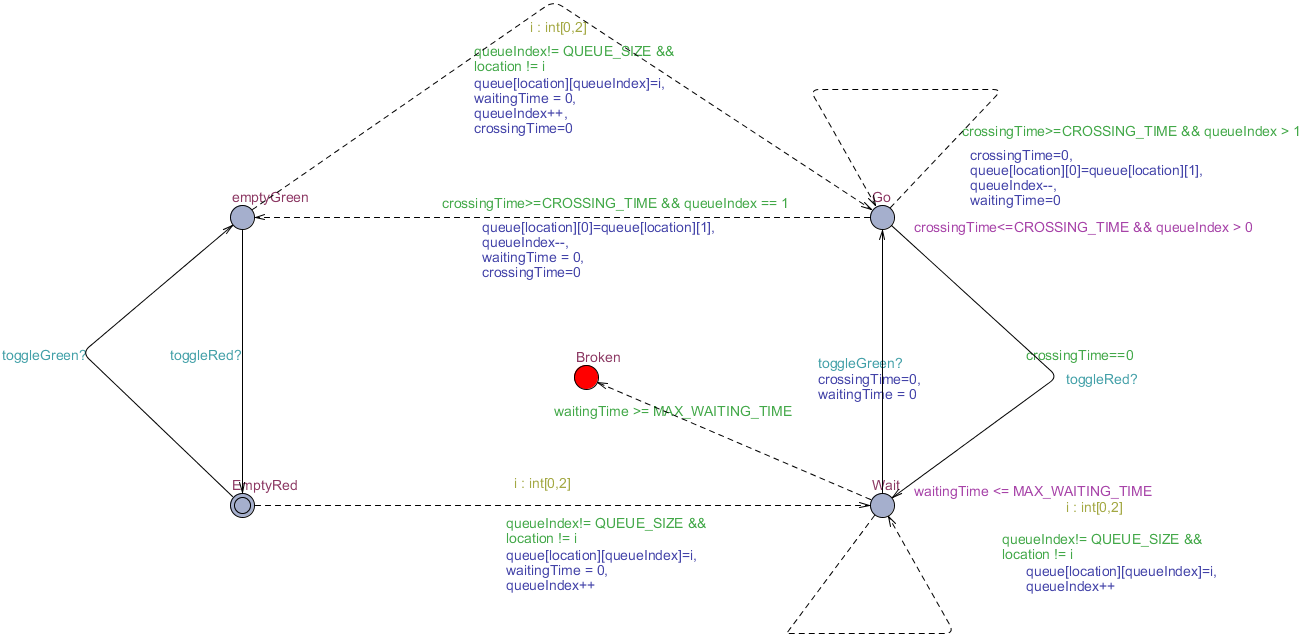
\includegraphics[width=\textwidth]{images/cargeneratort.png}
\end{figure}
\end{frame}

\begin{frame}{Dummy controller}
\begin{figure}[h]
\centering
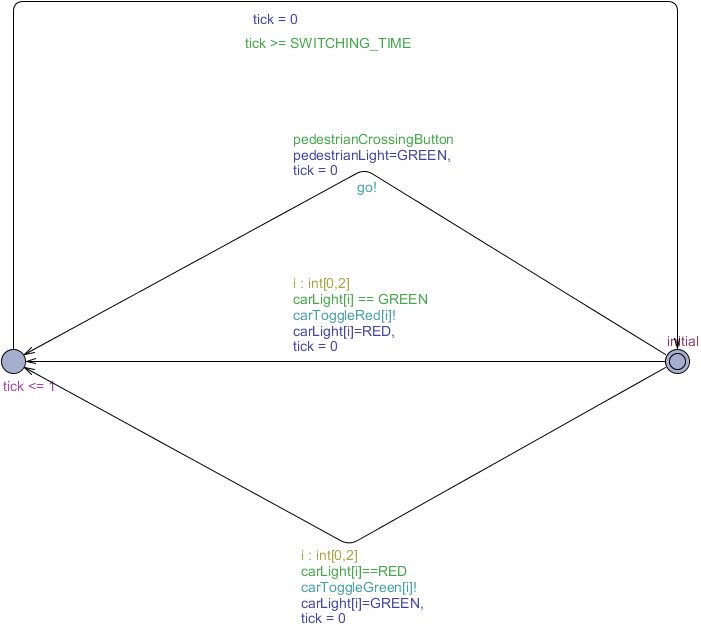
\includegraphics[width=0.75\textwidth]{images/controller.png}
\end{figure}
\end{frame}

\section{Winning condition}
\begin{frame}[fragile]{Winning condition}
\begin{alertblock}{}
Pure safety : the controler \textbf{must} avoid the losing states.
\begin{verbatim}
control : A[] not(lose)
\end{verbatim}
\end{alertblock}



\begin{block}{1. A pedestrian is never knocked down}
\begin{verbatim}
form_1 = 
control: A[] not(PedestrianGeneratorEast.Cross && 
(
    CarGeneratorEast.Go || 
    (
        CarGeneratorWest.Go && queue[W][0] == U
    ) || (
        CarGeneratorSouth.Go && queue[S][0] == R
    )))
\end{verbatim}
\end{block}

\end{frame}
\begin{frame}[fragile]{Winning condition}
\centering
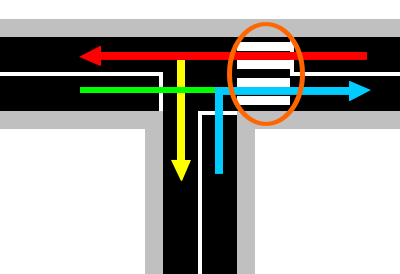
\includegraphics[scale=0.8]{images/pietonCollision.png}

\end{frame}


\begin{frame}[fragile]{Winning condition}
\begin{block}{2. Cars should never collide}
\begin{verbatim}
form_2 = 
Control: A[] not
(
    CarGeneratorWest.Go && queue[W][0] == U && 
    ((
        CarGeneratorEast.Go && queue[E][0] == L
    ) || (
        CarGeneratorSouth.Go && 
        ( queue[S][0] == L || queue[S][0] == R )
    ))
) || (
    CarGeneratorWest.Go && queue[W][0] == R 
    && CarGeneratorEast.Go && queue[E][0] == L
)
\end{verbatim}

Same idea for the two other orientations.
\end{block}

\end{frame}
\begin{frame}[fragile]{Winning condition}
\centering
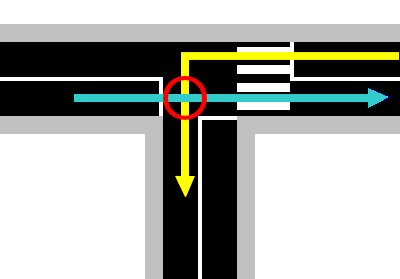
\includegraphics[scale=0.8]{images/exempleCollision.png}

\end{frame}


\begin{frame}[fragile]{Winning condition}
\begin{block}{3. Pedestrians do not wait infinitely}
\begin{verbatim}
form_3 = 
control: A[] not (PedestrianGeneratorEast.Broken)
\end{verbatim}
\end{block}

\begin{block}{4. Cars do not wait infinitely}
\begin{verbatim}
form_4 = 
control: A[] not (CarGeneratorEast.Broken ||
                  CarGeneratorSouth.Broken ||
                  CarGeneratorWest.Broken)
\end{verbatim}
\end{block}
\begin{block}{Full condition}
\begin{verbatim}
control: A[] not (
    form_1 || form_2 || form_3 ||form_4
)
\end{verbatim}
\end{block}
\end{frame} 

\section{Simulation}
\begin{frame}{Simulator}

\begin{block}{Base idea}
\begin{itemize}
\item Illustrate controller-environment interactions 
\item Environment behaves randomly
\item Controller avoids the bad states by implementing a winning strategy
\end{itemize}
\end{block}

\begin{block}{Problems}

\begin{itemize}
\item The winning strategy is huge ! 
\item It specifies a transition of the controller from each system state. 
\item Generate an execution trace from Uppaal tiga does not work (software problem)
\end{itemize}

\end{block}

\end{frame}

\begin{frame}{Simulator}

\begin{block}{Solution }
\begin{itemize}
\item Define a controller following a winning strategy in Uppaal (not tiga)
\item Then generate a trace of the whole system. 
\item Finally, convert this trace via the Libutap library (readable)
\end{itemize}
\end{block}

\begin{block}{GUI}
\begin{itemize}
\item Cars (bleu arrow), car lights (red arrow)
\item Pedestrians (yellow arrow), pedestrian light (green arrow)
\end{itemize}

\end{block}



\end{frame}

\begin{frame}{Simulator}

\centering
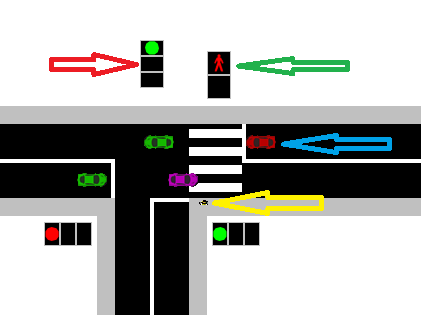
\includegraphics[scale=0.8]{images/SimP.PNG}

\end{frame}


\section{Conclusion}
\begin{frame}{Conclusion}

\begin{itemize}

\item The difficulty to model a system

\item The necessity to simplify the model to generate a winning strategy

\item The importance of choosing a good tool for our problem

\item The necessity to identify the different properties to satisfy

\item The necessity to identify the different actors which intervene in our problem

\item The difficulty to generate a winning strategy

\item The limit of the tools and how to extract a trace

\item This project allowed us to better understand the difficulty and the constraints which weigh on the modeling of a system

\item Little changes can increase a lot the number of states

\item The necessity to do compromises

\end{itemize}

\end{frame}
\end{document}
